
Fields are the basic data holding facilities in \libpniio\ and are represented
by instances of \nxfield. One can imagine a field as a multidimensional array 
stored on disk. Thus, it has quite similar properties than instances of 
\cpp{mdarray} in \libpnicore.  It is impossible to create a purely 
scalar field with \libpniio\ as every field should be extensible if required. 

%%%===========================================================================
\subsection{Creating fields}

Fields are created as children of a particular group instance. Creating fields
is a rather complex task as there are many options available so lets start with 
the simplest possible example
\begin{cppcode}
h5::nxgroup entry = root["entry"];
h5::nxfield field = entry.create_field<float32>("temperature");
\end{cppcode}
This creates a 1D field with a single element. This is as closest one can get 
to store a scalar value. The template parameter of the \cpp{create\_field}
method can be any type supported by \libpnicore.  For multidimensional fields
use 
\begin{cppcode}
h5::nxgroup entry = root["entry"];
h5::nxfield field = entry.create_field<float32>("temperature",shape_t{3,4});
\end{cppcode}
which will create a $2$-dimensional field with a shape of $(3,4)$ and a total
size of $12$ elements.
When using HDF5 as a storage format a compression algorithm can be associated
with a field. This algorithm will later on be used to compress the data stored
in a field and thus reduce disk utilization of the file. 
Currently only the standard deflate filter is supported 
\begin{cppcode}
h5::nxgroup entry = root["entry"];
h5::nxdeflate_filter deflate(4,false);
h5::nxfield field = entry.create_field<float32>("temperature",shape_t{3,4},deflate);
\end{cppcode}
In this particular case the filter uses a compression level of $4$ and no 
fletcher pre-sorting of the data. 

%%%===========================================================================
\subsection{Reading and writing data}

Fields provide two basic methods for reading and writing data: \cpp{read()} and
\cpp{write()}. Both member functions accept a single argument which can be an
instance of the following types
\begin{center}
    \begin{tabular}{l|p{0.6\linewidth}}
        {\bf type} & {\bf description} \\
        \hline
        \hline
        {\tt mdarray<...>} & an instance of the {\tt mdarray} template \\
        \hline
        {\tt array} & an instance of the array type erasure \\
        \hline
        {\tt T\& } & a single scalar value of the fields element type or a 
        convertible type \\
        \hline
    \end{tabular}
\end{center}
In addition there is a special version of \cpp{read()} and \cpp{write()}
available for legacy code with raw pointers. The two functions have the
signatures
\begin{cppcode}
template<typename T> void read(size_t n,T *ptr);
template<typename T> void write(size_t n,const T *ptr);
\end{cppcode}
The additional first argument \cpp{n} is the number of elements of type \cpp{T}
referenced by the pointer \cpp{*ptr}. This number ensures that the functions 
can check if the size of the field matches the number of elements which should
be read from or written to memory.
A scalar can be read from a field simply with
\begin{cppcode}
float32 temperature; 
h5::nxfield field = ...;
field.read(temperature);
\end{cppcode}
and writing runs exactly as one would expect
\begin{cppcode}
float32 temperator = ...;
h5::nxfield field = ...;
field.write(temperature);
\end{cppcode}
The same simple concept applies to all other types. For an instance of 
\cpp{mdarray} the code would look like this
\begin{cppcode}
auto data = dynamic_array<uint32>::create(shape_t{1024,1024});
h5::nxfield background = ....;

background.write(data); //writing

background.read(data);  //reading
\end{cppcode}

The \cpp{read()} and \cpp{write()} member functions perform a size check on
their arguments. The size of the argument must match the size of the field. 
In the case of scalar data a field-size of $1$ is assumed. If argument and field
size do not match a \cpp{size\_mismatch\_exception} is thrown.

%%%===========================================================================
\subsection{Growing fields}

\begin{figure}
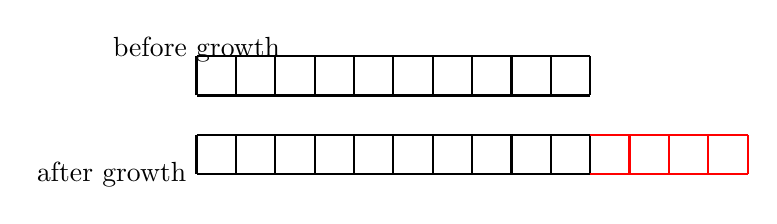
\begin{tikzpicture} [field/.style = {thick,step=5mm} ]
\draw[field] (0mm,0mm) node[anchor = east,above=3mm] {before growth} grid (50mm,5mm); 
\draw[field] (0mm,-10mm) node[anchor=east] {after growth} grid +(50mm,5mm);
\draw[field,color=red] (50mm,-10mm)  grid +(20mm,5mm);
\end{tikzpicture}
\end{figure}

The reason why there are no purely scalar fields is that during an experiment 
one would append data to a field as the measurement progresses. 
For this purpose \nxfield\ provides a \cpp{grow()} method which allows to 
extend the field along a particular dimension. The member function has the 
signature
\begin{cppcode}
void grow(size_t e,size_t n=1)
\end{cppcode}
where the first (mandatory) argument is the index of the dimension along which
the field should grow and the second (optional) argument contains the number of 
elements by which to grow. 

%%%===========================================================================
\subsection{Partial reading and writing}

Nexus fields support partial IO with the {\tt ()} operator which applies
selections to the field instances. 
\begin{cppcode}
h5::nxfield spectra = ...;

auto s = spectra.shape<shape_t>();

auto spectrum = dynamic_array<uint32>::create(shape_t{s[1]});

for(size_t i=0;i<s[0];++i)
{
    spectra(i,slice(0,s[1])).read(spectrum);
    .... process data ...
}
\end{cppcode}
The selection mechanism works the same as for the {\tt mdarray} template. 

%%%===========================================================================
\subsection{Field inquiry}
